%IMPORTS
\documentclass[a4paper, 11pt]{article}
\usepackage[utf8]{inputenc} 
\usepackage[T1]{fontenc}
\usepackage[catalan]{babel}
\usepackage{amsmath, amssymb, amsthm}
\usepackage[margin=1in]{geometry}
\usepackage{enumerate}
\usepackage{array}
\usepackage{graphicx}
\usepackage{wrapfig}
\usepackage{ragged2e} 
\usepackage{subfig}
\usepackage{caption}
\usepackage{subcaption}
\usepackage[dvipsnames]{xcolor}
%\usepackage[table]{xcolor}
\usepackage{float}
\usepackage{chngcntr}
\usepackage{ragged2e}
\usepackage{multirow}
\usepackage{vmargin}
\usepackage{hyperref}
\usepackage{url}
\usepackage{fancyhdr}
\usepackage{bigints}
\usepackage{listings}
\usepackage{xcolor,colortbl}
%\usepackage{slashbox}

\definecolor{navy}{rgb}{0,0,128}
\definecolor{codegreen}{rgb}{0,0.6,0}
\definecolor{codegray}{rgb}{0.5,0.5,0.5}
\definecolor{codepurple}{rgb}{0.58,0,0.82}
\definecolor{backcolour}{rgb}{0.95,0.95,0.92}
\definecolor{amaranth}{rgb}{0.9, 0.17, 0.31}
\definecolor{GRAY}{rgb}{0.75, 0.75, 0.75}

\lstdefinestyle{mystyle}{
    backgroundcolor=\color{white},   
    commentstyle=\color{codegreen},
    keywordstyle=\color{RoyalBlue},
    numberstyle=\tiny\color{codegray},
    stringstyle=\color{codepurple},
    basicstyle=\ttfamily\footnotesize,
    breakatwhitespace=false,         
    breaklines=true,                 
    captionpos=b,                    
    keepspaces=true,                 
    %numbers=left,                    
    numbersep=5pt,                  
    showspaces=false,                
    showstringspaces=false,
    showtabs=false,                  
    tabsize=2
}
\lstdefinestyle{Bash}
{language=bash,
keywordstyle=\color{blue},
basicstyle=\ttfamily,
morekeywords={peter@kbpet},
morekeywords=[2]{make},
keywordstyle=[2]{\color{blue}},
literate={\$}{{\textcolor{blue}{\$}}}1 
         {:}{{\textcolor{blue}{:}}}1
         {~}{{\textcolor{blue}{\textasciitilde}}}1,
}
\lstdefinestyle{BASH}
{language=bash,
keywordstyle=\color{blue},
basicstyle=\ttfamily,
morekeywords={peter@kbpet},
morekeywords=[2]{make},
fontsize=5pt
keywordstyle=[2]{\color{blue}},
literate={\$}{{\textcolor{blue}{\$}}}1 
         {:}{{\textcolor{blue}{:}}}1
         {~}{{\textcolor{blue}{\textasciitilde}}}1,
}

\lstset{style=mystyle}

\setpapersize{A4}
\setmargins{2.5cm}     % margen izquierdo
{2.6cm}                % margen superior
{16.5cm}               % anchura del texto
{23.7cm}               % altura del texto
{10pt}                 % altura de los encabezados
{0cm}                  % espacio entre el texto y los encabezados
{0pt}                  % altura del pie de página
{1cm}                  % espacio entre el texto y el pie de página
\renewcommand{\baselinestretch}{1.5}

\begin{document}

\begin{titlepage}
    \centering
    {\bfseries\LARGE Universitat Autònoma de Barcelona\newline Facultat de Ciències\par}
    \vspace{2cm}
    {\hspace{-1em}
\includegraphics[width=0.4\textwidth]{logo.png}\par}
    \vspace{1cm}
    {\scshape\Huge Pràctica 2\par} 
    \vspace{1cm}
    {\Large \itshape Autors: \par}
    {\Large \hspace{-1.75em} Gerard Lahuerta \& Ona Sánchez \par}
    {\Large 1601350 --- 1601181 \par}
    \vspace{1cm}
    {\Large 29 de Abril del 2022\par}
\end{titlepage}

\justifying

\newpage
\setcounter{page}{2}
\pagestyle{plain}
\tableofcontents
\cleardoublepage
\addcontentsline{}{chapter}{}
\newpage
\section{Presentació de la llibreria i informació d'interés}\label{pres.llib}
La llibreria de funcions ha estat programada en llenguatge $C$ i consta de tres fitxers, un fitxer capcelera i dos amb el codi de les funcions.\\
Aquests dos fitxers amb codi: un que precisa de la llibreria \textcolor{LimeGreen}{gsl\_rng.h} per al seu funcionament, i un altre que usa \textcolor{LimeGreen}{math.h}, \textcolor{LimeGreen}{limits.h}, \textcolor{LimeGreen}{stdlib.h}.\\ 
El fitxer capcelera, per contra, es comú als dos fitxers.\\
També, els fitxers capcelera tenen definides les constants:
\begin{itemize}
    \item \textcolor{Dandelion}{E\_INTER}: missatge d'error per valor inferior del interval major al superior.
    \item \textcolor{Dandelion}{E\_SIGMA}: missatge d'error per $\sigma^2 \leq 0 $.
\end{itemize}
La llibreria té programades tres funcions, on dues permeten generar nombres aleatoris (cadascuna amb una distribució diferent). Ambdues retornen un sol valor aleatori, que és de tipus \textbf{\textcolor{Turquoise}{double}}. La tercera funció permet inicialitzar la llavor de generació dels nombres aleatoris.\\
Recalcar a més, que cada funció conté el seu $CDocs$ propi que conté la informació més rellevant de la funció de manera resumida: \textit{input, output, descripció} i \textit{informació rellevant}.\\ 
Per finalitzar, comentar que s'ha decidit crear un segon fitxer per a la utilització de la llibreria \textcolor{LimeGreen}{gsl\_rng.h}.\\
Cal mencionar que el programa $gauss.c$ ha sigut modificat, de manera que fa ús exclusiu de la funció \textbf{\textcolor{blue}{Simpson}} per calcular $P(|X| > |x|) \leq p$.

\newpage
\section{Presentació de les funcions}
\subsection{Fitxer aleatori.c} \label{aleatori}
\subsubsection{init\_seed}
\begin{itemize}
    \item Entrada: Llavor, \textbf{\textcolor{Turquoise}{double}} seed.
    \item Sortida: No retorna cap valor, \textbf{\textcolor{Turquoise}{void}}.
    \item Funcionament:
    Inicialitza els mètodes de generació aleatoris de la llibreria \textcolor{LimeGreen}{stdlib.h} mitjançant la funció \textbf{\textcolor{blue}{srand}}, introduïnt-li per argument la llavor que rep el mètode.
\end{itemize}


\subsubsection{Uniforme}
\begin{itemize}
    \item Entrada:
    \begin{itemize}
        \item[$\circ$] Valor inferior de l'interval: \textbf{\textcolor{Turquoise}{double}} $a$.
        \item[$\circ$] Valor superior de l'interval: \textbf{\textcolor{Turquoise}{double}} $b$.
    \end{itemize}
    \item Sortida:
        \begin{itemize}
            \item[$\circ$] Nombre aleatori dins l'interval $[a,b]$:  \textbf{\textcolor{Turquoise}{double}}.
        \end{itemize}
    \item Funcionament:
    Un cop cridada la funció amb els paràmetres corresponents, s'usa la funció \textbf{\textcolor{blue}{rand}} per generar un nombre aleatori a l'interval $[0,1]$ i el següent canvi de variable per retornar un nombre aleatori dins l'interval desitjat: $rnd \cdot (b-a) + a $, on $rnd$ és un nombre aleatori de l'interval $[0,1]$.
    
\end{itemize}
\newpage
\subsubsection{Normal} \label{normalnormal}
\begin{itemize}
    \item Entrada:
    \begin{itemize}
        \item[$\circ$] Valor de l'esperança de la normal: \textbf{\textcolor{Turquoise}{double}} mu.
        \item[$\circ$] Valor de la variànça de la normal: \textbf{\textcolor{Turquoise}{double}} sigma.
    \end{itemize}
    \item Sortida:
        \begin{itemize}
            \item[$\circ$] Nombre aleatori que segueix una distribució $\mathcal{N}(\mu,\,\sigma^{2})$:  \textbf{\textcolor{Turquoise}{double}}.
        \end{itemize}
    \item Funcionament:
    Un cop cridada la funció amb els paràmetres corresponents, es crida la funció \textbf{\textcolor{blue}{Uniforme}}, amb els paràmetres $-1$ i $1$, per generar una parella de nombres aleatoris $u, v$ uniformes a $[-1,1]$ tals que $s = u^2 + v^2 < 1$. De manera aleatòria es selecciona \textbf{un} dels següents nombres aleatoris que segueixen una $\mathcal{N}(0,1)$:
    
    \begin{equation*}
        n_{1} = u\sqrt{\frac{-2\log(s)}{s}}
    \end{equation*}
    \begin{equation*}
        n_{2} = v\sqrt{\frac{-2\log(s)}{s}}
    \end{equation*}
    
\end{itemize}
Se li aplica al valor seleccionat el següent canvi de variable: $n_{i}\cdot s \cdot sigma+mu$, de manera que es retorna un valor aleatori que segueix una $\mathcal{N}(\mu,\,\sigma^{2})$.
\newpage
\subsection{Fitxer aleatori\_gsl.c} \label{aleatorigsl}
Mencionar que el fitxer $aleatori\_gsl.c$ conté declarades les variables globals \textcolor{cyan}{\textit{T}} i  \textcolor{cyan}{\textit{rng}}.
\subsubsection{init\_seed}
\begin{itemize}
    \item Entrada: Llavor, \textbf{\textcolor{Turquoise}{double}} seed.
    \item Sortida: No retorna cap valor, \textbf{\textcolor{Turquoise}{void}}.
    \item Funcionament:
    Crea l'estructura \textcolor{cyan}{\textit{rng}} de la llibreria  \textcolor{LimeGreen}{gsl\_rng.h} encarregada de generar els nombres aleatoris mitjançant la llavor introduïda com a paràmetre.
\end{itemize}
\subsubsection{Uniforme}
\begin{itemize}
    \item Entrada:
    \begin{itemize}
        \item[$\circ$] Valor inferior de l'interval: \textbf{\textcolor{Turquoise}{double}} a.
        \item[$\circ$] Valor superior de l'interval: \textbf{\textcolor{Turquoise}{double}} b.
    \end{itemize}
    \item Sortida:
        \begin{itemize}
            \item[$\circ$] Nombre aleatori dins l'interval [a,b]:  \textbf{\textcolor{Turquoise}{double}}.
        \end{itemize}
    \item Funcionament:
    Usa la funció \textbf{\textcolor{blue}{gsl\_rng\_uniform}}$($\textcolor{cyan}{\textit{rng}}$)$ per generar un nombre aleatori a l'interval $[0,1]$ i el següent canvi de variable per retornar un nombre aleatori dins l'interval desitjat: $rnd \cdot (b-a) + a $ on $rnd$ és el valor retornat per per la funció anteriorment mencionada.
    
\end{itemize}




\newpage
\subsubsection{Normal}
\begin{itemize}
    \item Entrada:
    \begin{itemize}
        \item[$\circ$] Valor de l'esperança de la normal: \textbf{\textcolor{Turquoise}{double}} mu.
        \item[$\circ$] Valor de la variànça de la normal: \textbf{\textcolor{Turquoise}{double}} sigma.
    \end{itemize}
    \item Sortida:
        \begin{itemize}
            \item[$\circ$] Nombre aleatori que segueix una distribució $\mathcal{N}(\mu,\,\sigma^{2})$:  \textbf{\textcolor{Turquoise}{double}}.
        \end{itemize}
    \item Funcionament:
    Segueix el procediment explicat anteriorment a l'apartat \textcolor{blue}{\ref{normalnormal}}. Es fan dues crides a la funció \textbf{\textcolor{blue}{Uniforme}} que usa el mètode de la gsl per retornar un nombre aleatori.
\end{itemize}




\newpage
\section{Control dels errors}
\subsection{Llibreries: $aleatori.c$ i $aleatori\_gsl.c$}
Per tal d'assegurar el correcte funcionament dels mètodes implementats a les llibreries a inicis de la funció (abans de començar a fer cap càlcul) es confirmarà la correcta introducció dels paràmetres.\\
Es comprovarà:
\begin{enumerate}
    \item Que el valor inferior de l'interval sigui menor al superior (en la funció \textcolor{blue}{Uniforme}).
    \item Que el valor $\sigma^2$ introduït sigui estrictament positiu (en la funció \textcolor{blue}{Normal}).
\end{enumerate}
En cas d'inclompir alguna d'aquestes condicions el programa actuarà de la següent manera:
\begin{itemize}
    \item Es mostrarà per pantalla el missatge d'error corresponent, guardat a la variable \textcolor{Dandelion}{E\_ITER} o \textcolor{Dandelion}{E\_SIGMA} (explicades anteriorment a la secció \textcolor{blue}{\textbf{\ref{pres.llib}}}).
\end{itemize}
Recalcar que en cas d'inclomplir alguna condició que impedexi fer els càlculs (cas que no es compleixin les condicions $1$ o $2$) es retornarà el valor $LLONG\_MAX$.
\newpage
\subsection{Programa $generador.c$}\label{com_er}
Per tal d’assegurar el correcte funcionament del programa es confirmarà la correcta introducció
dels paràmetres de la següent forma:
\begin{enumerate}
    \item Es comprova que s'hagin introduït els dos paràmetres necessaris ($\mu$, $\sigma^2$). És retornarà el valor $-1$ en cas que no es compleixi la condició.
    \item Es comprova que el valor de sigma sigui positiu. Es retornarà el valor $-2$ en cas que no es compleixi la condició.
    \item Si s'introdueix un valor més, es guarda a la variable $n$ (nombre de números aleatoris a generar), sempre i quan sigui major a $0$. Si s'introdueix un valor decimal, es guardarà el valor enter més proper arrodonint cap avall.
    \item Si s'introdueix un valor més, es guarda a la variable $seed$.
    \item Tota la resta d'arguments entrats seran obviats.
    \item En cas de no haver-se produït cap error, es retornarà un $0$.
\end{enumerate}
\vspace{2em}
\subsection{Programa $comprovador.sh$}
Per tal d’assegurar el correcte funcionament del programa a l’inici de la funció (abans de
començar a fer cap càlcul) es confirmarà la correcta introducció dels paràmetres de la següent
forma:

\begin{enumerate}
    \item Es comprova que s'hagi introduït el paràmetre necessari $p$ i que aquest pertanyi a l'interval $[0,1]$.
    \item Si s'introdueixen més paràmetres, es guarden a les variables $\mu$, $\sigma^2$, $n$ i $seed$ respectivament.
    \item Si s'afegeix un sisè paràmetre (nombre d'intervals pel mètode de Simpson), es comprova que el valor sigui positiu i diferent de $0$, en cas contrari, no es guardarà i quedarà el valor per defecte, $300$.
\end{enumerate}
\newpage
\section{Compilació i execució}
\subsection{Compilació del Programa} \label{compilacio}
\subsubsection{Makefile}
Per facilitar la compilació dels programes s'ha creat un fitxer $makefile$ que inclou tant les comandes per crear els executables com altres comandes associades (que explicarem més endavant) per la correcta gestió dels fitxers que s'obtenen de l'execució del makefile.\\\\
Per poder executar el fitxer $makefile$ cal abans modificar el fitxer d'opcions amb els \textit{path} correctes d'on es troba la carpeta $gsl$ que conté totes les seves llibreries.\\
El fitxer d'opcions s'anomena $options.mk$ i s'han de modificar les variables \textcolor{amaranth}{INCLUDEPATH} i \textcolor{amaranth}{LIBPATH} amb els path correctes (path on es troba la carpeta $gsl$ i path on es troba la carpeta $libgsl.so.xx$ on $xx$ és la versió de la llibreria $gsl$ respectivament).\\\\
Mencionar que no es poden utilitzar dues comandes "\textit{clean}"\hspace{0.4em}de manera seguida ja que donarà error.\\\\
\textbf{Important:} en cas de no utilitzar el sistema operatiu $Linux$ (o semblants) o $IOS$ cal modificar la variable \textcolor{amaranth}{DELETE} de l'arxiu $options.mk$ per a poder utilitzar-lo (substituir per la comanda $del$ en cas d'utilitzar Windows).
\newpage
\hspace{-1.5em}Per compilar el programa, generar els executables i gestionar els fitxers creats, hem creat les següents rutines, podem executar les comandes:\\
\begin{table}[h]
    \centering
    \begin{tabular}{l|l}
        \textbf{Comanda} & \textbf{Descripció} \\ \hline \hline 
        \multirow{2}{*}{ \textcolor{blue}{\$make}} & Compila el programa i genera els \\
        & executables $gauss$, $generador$ i $comprovador.sh$.\\ \hline
        \multirow{2}{*}{ \textcolor{blue}{\$make} gauss} & Compila el programa i genera \\
        & l'executable corresponent ($gauss$). \\\hline
        \multirow{3}{*}{ \textcolor{blue}{\$make} generador} & Compila el programa i genera \\
        & l'executable corresponent ($generador$)\\ 
        & mitjançant el fitxer $aleatori.c$. \\ \hline
        \multirow{3}{*}{ \textcolor{blue}{\$make} generador\_gsl} & Compila el programa i genera l'executable \\
        & corresponent ($generador$)\\
        & utilitzant el fitxer $aleatori\_gsl.c$\\\hline
        \multirow{2}{*}{ \textcolor{blue}{\$make} comprovador.sh} & Canvia els permisos del fitxer $comprovador.sh$\\
        & per a que es pugui executar.\\\hline
        \multirow{2}{*}{\textcolor{white}{l}\textcolor{blue}{\$make} clean} & Elimina tots el fitxers amb \\
        & terminació $.o$ del directori.\\\hline
        \multirow{2}{*}{ \textcolor{blue}{\$make} clean\_gauss} & Elimina l'executable $gauss$ i els \\
        & fitxers generats amb terminació $.o$. \\\hline
        \multirow{2}{*}{ \textcolor{blue}{\$make} clean\_generador} & Elimina tant l'executable $generador$\\
        & com els fitxers generats amb terminació $.o$.\\\hline
        \multirow{2}{*}{ \textcolor{blue}{\$make} clean\_all} & Elimina tant tots els executables \\
        & com els fitxers amb terminació $.o$. \\
        
    \end{tabular}
    \label{tab:my_label}
\end{table}\\

\hspace{-1.5em}\textbf{Important:} En executar la comanda $make$ es compilarà l'executable $generador$ utilitzant el fitxer $aleatori.c$.

\newpage
\subsubsection{Compilació manual}
Recomanem utilitzar en ordre les comandes que mostrarem al terminal (una vegada ubicat al directori on es troben els fitxers).
\begin{itemize}
    \item \textbf{Compilació del programa $gauss$}\\
    Recomanem llegir \textcolor{blue}{\href{https://www.overleaf.com/read/dncxfhyjpjgv}{l'apartat de compilació manual de la pràctica 1 (5.1.2)}}.
    
    \item \textbf{Compilació del programa $generador$}\\
    \begin{itemize}
        \item Compilació amb $aleatori.c$
        \begin{lstlisting}[language=BASH]
gcc -c aleatori.c aleatori.h -lm
gcc -c generador.c  aleatori.c -lm
gcc generador.o  aleatori.o -lm -o generador
        \end{lstlisting}
        \item Compilació amb $aleatori\_gsl.c$
        \begin{lstlisting}[language=BASH]
gcc -c aleatori_gsl.c aleatori.h -I$(INCLUDEPATH) -lm
gcc -c generador.c  aleatori_gsl.c -I$(INCLUDEPATH) -lm
gcc generador.o aleatori_gsl.o -L$(LIBPATH) -Wl,-R$(LIBPATH) -lgsl 
                               -lgslcblas -lm -o generador
        \end{lstlisting}
    \end{itemize}

    \item \textbf{Modificació dels permisos del shell script $comprovador.sh$}
    \begin{lstlisting}[language=BASH]
    chmod 744 comprovador.sh
    \end{lstlisting}
\end{itemize}


\newpage

\subsection{Execució del Programa}
Per a una millor utilització i gestió dels programes, hem fet tots els nostres programes suficientment flexibles com per a que s'adaptin a les necessitats que es poden tenir sense accedir i/o modificar el codi. Per això es poden executar de diverses maneres; mostrem ara una taula amb totes les possibles execucions dels nostres programes.
\subsubsection{Execució del programa $generador$}\label{exe_gen}
\begin{table}[h]
    \centering
    \begin{tabular}{l|l}
        \textbf{Comanda} & \textbf{Descripció} \\ \hline \hline 
        \multirow{2}{*}{\texttt{./generador $\mu$ $\sigma^2$ }} & Genera 2 milions de nombres aleatoris que segueixen una  \\
        & $\mathcal{N}(\mu,\,\sigma^{2})$, usant una llavor aleatòria. \\\hline
        \multirow{2}{*}{\texttt{./generador $\mu$ $\sigma^2$ n }} & Genera $n$ nombres aleatoris que segueixen una $\mathcal{N}(\mu,\,\sigma^{2})$,\\
        & usant una llavor aleatòria.\\\hline
        \multirow{2}{*}{\texttt{./generador $\mu$ $\sigma^2$ n seed}}  & Genera $n$ nombres aleatoris que segueixen una $\mathcal{N}(\mu,\,\sigma^{2})$, \\
        &usant la llavor seed. \\
        
    \end{tabular}
    \label{tab:my_label}
\end{table}
\hspace{-1.5em}Qualsevol argument de més que s'introdueixi al programa serà omés.\\\\
Recalcar que tant si és compilat amb el fitxer $aleatori.c$ com amb el fitxer $aleatori\_gsl.c$ el funcionament i execució del programa generador és el mateix; només varia la forma de generar nombres pseudo-aleatoris.\\\\
\textbf{IMPORTANT:} Si a l'hora d'executar el programa $generador$ compilat amb el fitxer 
\\$aleatori\_gsl.c$ apareix l'error: \texttt{error while loading shared libraries libgsl.so.xx} on $xx$ és la versió del $gsl$ o algun error semblant, pot ser degut a un d'aquest dos casos:
\begin{enumerate}
    \item Les variables \textcolor{amaranth}{INCLUDEPATH} i/o \textcolor{amaranth}{LIBPATH} no contenen el \textit{path} correcte. Cal revisar el \textit{path} que guarden.
    \item L'executable no accedeix correctament a la llibreria $gsl$. Cal executar al terminal la comanda següent: \textcolor{blue}{\$export} PATH, on PATH és una variable que conté el mateix path que \textcolor{amaranth}{LIBPATH} i ha sigut declarada al terminal, prèviament a la recompilació i reexecució del programa.
\end{enumerate}
\newpage


\newpage
\section{Comprovacions de funcionament} \label{comprovacions}
\subsection{Programa $generador.c$}
Recordem que el programa $generador.c$ és l'encarregat de generar una mostra de nombres aleatoris mitjançant la llibreria \textcolor{LimeGreen}{aleatori.h}. \\
Recomanem haver llegit amb anterioritat les seccions \textcolor{blue}{\ref{aleatori}} i \textcolor{blue}{\ref{exe_gen}} (per a les diverses formes de generació de nombres aleatoris, $aleatori.c$ i $aleatori\_gsl.c$, i les diverses formes d'executar el programa).\\
Fem énfasis en que cal llegir l'aparat \textcolor{blue}{\ref{compilacio}} en cas de tenir algun dubte sobre com compilar degudament el programa.\\\\
%errors veure k van
%probar x semilla per veure que surt lo k toca
Per tal d'asegurar el correte funcionament del programa, adjuntem aquí un seguit d'instruccions per comprovar que actui de la manera desitjada.\\\\
Recalcar que s'ha utilitzat el fitxer $aleatori.c$ per generar la mostra de nombres aleatoris, les excepcions estan indicades i quan s'ha utilitzat el fitxer $aleatori\_gsl.c$ s'ha fet mitjançant la versió $2.7$ de la llibreria de funcions $gsl$.
\newpage
\begin{itemize}
    \item Execució per la comanda \texttt{./generador $\mu$ $\sigma^2$}\\
    \begin{table}[h]
            \begin{center}
            \begin{tabular}{ l | l }
            \textbf{Comanda} & \textbf{Output}\\ \hline\hline
            \texttt{./generador } & \texttt{./generador mu sigma}\\ \hline
            \multirow{2}{*}{\texttt{./generador  $0$ $-1$}} & \texttt{The value of sigma squared has} \\
            & \texttt{to be positive (more than 0)}\\ \hline
            \multirow{6}{*}{\texttt{./generador $-1$  $1$}} & \hspace{2em}\texttt{    mu} \hspace{0.2em}\texttt{  sigma            }\hspace{5.9em}\texttt{x}\\ 
            & \texttt{-1.0000 1.0000 0.281100657152}\\
            & \texttt{-1.0000 1.0000 0.799279379685}\\
            & \texttt{-1.0000 1.0000 -1.165641526839}\\
            & \texttt{-1.0000 1.0000 -0.609642695197}\\
            & \hspace{2.5em}$\vdots$ \hspace{3em}$\vdots$ \hspace{5.5em}$\vdots$\\\hline
            \multirow{6}{*}{\texttt{./generador  $0$  $1$}} & \hspace{1.5em}\texttt{    mu} \hspace{0.2em}\texttt{  sigma            }\hspace{5.9em}\texttt{x}\\ 
            & \texttt{0.0000 1.0000 -0.873712043554}\\
            & \texttt{0.0000 1.0000 0.378018969177}\\
            & \texttt{0.0000 1.0000 -0.681342010392}\\
            & \texttt{0.0000 1.0000 -1.982028443212}\\
            & \hspace{2.5em}$\vdots$ \hspace{3em}$\vdots$ \hspace{5.5em}$\vdots$\\
            \end{tabular}
            \end{center}
    \end{table}\\
    Fem énfasi que els valors que s'obtenen de les comandes superiors estan generats per una llavor aleatòria pel que si es repeteix la comanda és possible que no s'obtinguin els mateixos valors.\\
    Si es volen comparar els valors que s'obtenen amb alguna de les mostres cal introduir la mateixa llavor (cas que es mostrarà amb posterioritat).
    \end{itemize}
    \newpage
    \begin{itemize}
    \item Execució per la comanda \texttt{./generador $\mu$ $\sigma^2$ $n$}\\
    \begin{table}[h]
            \begin{center}
            \begin{tabular}{ l | l }
            \textbf{Comanda} & \textbf{Output}\\ \hline\hline
            \multirow{4}{*}{\texttt{./generador  $0$  $1$ $0$}} & \hspace{1.5em}\texttt{    mu} \hspace{0.2em}\texttt{  sigma            }\hspace{5.9em}\texttt{x}\\ 
            & \texttt{0.0000 1.0000 -0.725798830034}\\
            & \texttt{0.0000 1.0000 0.945648247014}\\
            & \hspace{2.5em}$\vdots$ \hspace{3em}$\vdots$ \hspace{5.5em}$\vdots$\\\hline
             \multirow{6}{*}{\texttt{./generador  $0$  $1$ $3$}} &\texttt{The value of numbers requested}\\
             & \texttt{has changed to 3} \\
             & \hspace{1.5em}\texttt{    mu} \hspace{0.2em}\texttt{  sigma            }\hspace{5.9em}\texttt{x}\\  
            & \texttt{0.0000 1.0000 -0.886783121527}\\
            & \texttt{0.0000 1.0000 0.807136605579}\\
            & \texttt{0.0000 1.0000 1.354447153111}\\\hline
             \multirow{4}{*}{\texttt{./generador  $0$  $1$ $-3$}} & \hspace{1.5em}\texttt{    mu} \hspace{0.2em}\texttt{  sigma            }\hspace{5.9em}\texttt{x}\\ 
            & \texttt{0.0000 1.0000 1.515762223841}\\
            & \texttt{0.0000 1.0000 2.500994297887}\\
            & \hspace{2.5em}$\vdots$ \hspace{3em}$\vdots$ \hspace{5.5em}$\vdots$\\\hline
             \multirow{6}{*}{\texttt{./generador  $0$  $1$ $3.1$}} &\texttt{The value of numbers requested}\\
             & \texttt{has changed to 3} \\
             & \hspace{1.5em}\texttt{    mu} \hspace{0.2em}\texttt{  sigma            }\hspace{5.9em}\texttt{x}\\ 
            & \texttt{0.0000 1.0000 -0.418507079666}\\
            & \texttt{0.0000 1.0000 1.128969639183}\\
            & \texttt{0.0000 1.0000 0.045605789271}\\
            \end{tabular}
            \end{center}
    \end{table}\\
    Com ja s'ha explicat, en cas d'introduir un valor per al paràmatre $n\in(-\infty,0]$ el programa ignorarà el valor i assignarà a $n$ el valor $2000000$.\\
    En cas de dubtes sobre els controls d'errors del programa $generador.c$ cal llegir la secció \textcolor{blue}{\ref{com_er}}
    \end{itemize}
    \newpage
    \begin{itemize}
    \item Execució per la comanda \texttt{./generador $\mu$ $\sigma^2$ $n$ $seed$}
        \begin{table}[h]
            \begin{center}
            \begin{tabular}{ l | l }
            \textbf{Comanda} & \textbf{Output}\\ \hline\hline
             \multirow{9}{*}{\texttt{./generador  $0$  $1$ $5$ $6$}} &\texttt{The value of numbers requested}\\
             & \texttt{has changed to 5} \\
             & \texttt{The seed for random generation }\\
             & \texttt{has been changed by 6.000000}\\
             &\hspace{1.5em}\texttt{    mu} \hspace{0.2em}\texttt{  sigma            }\hspace{5.9em}\texttt{x}\\ 
            & \texttt{0.0000 1.0000 -0.418507079666}\\
            & \texttt{0.0000 1.0000 1.128969639183}\\
            & \texttt{0.0000 1.0000 0.045605789271}\\
            & \texttt{0.0000 1.0000 -0.422646654265}\\
            & \texttt{0.0000 1.0000 0.067429724966}\\\hline
             \multirow{9}{*}{\texttt{./generador  $0$ $1$ $5$ $6$ $others$}} &\texttt{The value of numbers requested}\\
             & \texttt{has changed to 5} \\
             & \texttt{The seed for random generation }\\
             & \texttt{has been changed by 6.000000}\\
             & \hspace{1.5em}\texttt{    mu} \hspace{0.2em}\texttt{  sigma            }\hspace{5.9em}\texttt{x}\\ 
            & \texttt{0.0000 1.0000 -0.418507079666}\\
            & \texttt{0.0000 1.0000 1.128969639183}\\
            & \texttt{0.0000 1.0000 0.045605789271}\\
            & \texttt{0.0000 1.0000 -0.422646654265}\\
            & \texttt{0.0000 1.0000 0.067429724966}\\
            \end{tabular}
            \end{center}\label{taula1}
    \end{table}
    \end{itemize}
    Podem observar que, com cal esperar, en introduir el mateix valor a la variable $seed$ ($6$, en el cas de la taula mostrada) s'obtenen resultats idèntics.\\
    També es pot veure que en introduir més paràmetres ($others$), el programa els ignora i actua com si no hi fossin.
    \newpage
\begin{itemize}
    \item Execució amb la llibreria $gsl\_rng$
     \begin{table}[h]
            \begin{center}
            \begin{tabular}{ l | l }
            \textbf{Comanda} & \textbf{Output}\\ \hline\hline
             \multirow{4}{*}{\texttt{./generador  $0$  $1$ }} 
             &\hspace{1.5em}\texttt{    mu} \hspace{0.2em}\texttt{  sigma            }\hspace{5.9em}\texttt{x}\\ 
            & \texttt{0.0000 1.0000 -0.710010616221}\\
            & \texttt{0.0000 1.0000 -0.492539236371}\\
            & \hspace{2.5em}$\vdots$ \hspace{3em}$\vdots$ \hspace{5.5em}$\vdots$\\
            \hline
            
             \multirow{6}{*}{\texttt{./generador  $0$ $1$ $3$ }} &\texttt{The value of numbers requested}\\
             & \texttt{has changed to 3} \\
             &\hspace{1.5em}\texttt{    mu} \hspace{0.2em}\texttt{  sigma            }\hspace{5.9em}\texttt{x}\\ 
            & \texttt{0.0000 1.0000 0.178299690868}\\
            & \texttt{0.0000 1.0000 0.611195213845}\\
            & \texttt{0.0000 1.0000 0.739190745288}\\
            \hline
            
            \multirow{8}{*}{\texttt{./generador  $0$  $1$ $3$ 
            $6$}} &\texttt{The value of numbers requested}\\
             & \texttt{has changed to 3} \\
             & \texttt{The seed for random generation }\\
             & \texttt{has been changed by 6.000000}\\
             &\hspace{1.5em}\texttt{    mu} \hspace{0.2em}\texttt{  sigma            }\hspace{5.9em}\texttt{x}\\ 
            & \texttt{0.0000 1.0000 0.931214928923}\\
            & \texttt{0.0000 1.0000 0.413912021687}\\
            & \texttt{0.0000 1.0000 0.527323084343}\\
            \end{tabular}
            \end{center}
    \end{table}
\end{itemize}
Com es pot observar, en introduir els valors $\mu$, $\sigma^2$ es genera un fitxer (que ocupa $200000$ de linies), del qual es mostren les primeres files.\\
En afegir el valor de la $n$, es genera un fitxer de $n$ linies.\\
Destacar que els valors obtinguts han estat generats per una llavor aleatòria pel que en executar aquestes mateixes comandes, s'obtindran resultats diferents.\\
A la tercera comanda, en canvi, la llavor ha sigut introduïda per paràmetre ($6$), de manera que si s'executa aquesta mateixa comanda un altre cop, donarà resultats idèntics.\\
També es veu com (mitjançant la mateixa llavor que anteriorment) es generen nombres aleatoris diferents, ja que el mètode de generació es diferent amb la llibreria $gsl$ que amb els mètodes implementats per nosaltres (resultats de la taula de la pàgina \textcolor{blue}{ \pageref{taula1}}). \\
La informació en detall es mostra a les seccions: \textcolor{blue}{\ref{aleatori}}, \textcolor{blue}{\ref{aleatorigsl}} i \textcolor{blue}{\ref{compilacio}}

\newpage
\subsection{Shell script $comprovador.sh$}
Recordem que el programa $comprovador.sh$ és l'encarregat de crear un fitxer (que s'anomena automàticament $random\_samples.txt$), que guarda a cada linia els valors $\mu$, $\sigma^2$ i $x$, on $x$ és el nombre aleatori que segueix una distribució $\mathcal{N}(\mu,\,\sigma^{2})$, resultant d'una crida al programa $generador.c$ explicat anteriorment.\\
Per a l’execució i introducció de les dades es recomana llegir l’apartat anterior \textcolor{blue}{\ref{excomprovador}}.\\
Per a la correcta compilació del programa recomanem llegir l'apartat \textcolor{blue}{\ref{compilacio}}.\\\\
Per tal d’asegurar el correte funcionament del programa, adjuntem aquí un seguit d’instruccions per tal de comprovar que el programa actui de la manera desitjada.

\begin{itemize}
    \item Execució per la comanda \texttt{./comprovador $p$}
    \begin{table}[h]
            \begin{center}
            \begin{tabular}{ l | l | l}
            \textbf{Comanda} & \textbf{Output} & \textbf{Fragment $random\_samples.txt$}\\ \hline\hline
            \multirow{2}{*}{\texttt{./comprovador.sh }} & Argument of the probability &\multirow{2}{*}{\cellcolor{GRAY}{}\textcolor{GRAY}{HHHHHHHHHHHHHHHHHHHHH} }\\ 
            &p is missing &   \cellcolor{GRAY}{}\\ \hline
            \multirow{2}{*}{\texttt{./comprovador.sh 2}} & Argument of the probability &  \multirow{2}{*}{\cellcolor{GRAY}{}\textcolor{GRAY}{HHHHHHHHHHHHHHHHHHHHH} }\\
            &has to be between 0 and 1 & \cellcolor{GRAY}{}\\ \hline
            \multirow{3}{*}{\texttt{./comprovador.sh 0.3}} & The number of samples x with & 0.0000 1.0000 -0.666410103803\\
            &probability&  0.0000 1.0000 0.543107721219\\
            &P(|X| > |x| ) $\leq$ p is 600437& \hspace{1.5em}$\vdots$ \hspace{2.5em}$\vdots$ \hspace{4.5em}$\vdots$ \\ \hline
            \multirow{2}{*}{\texttt{./comprovador.sh -0.3}} & Argument of the probability &  \multirow{2}{*}{\cellcolor{GRAY}{}\textcolor{GRAY}{HHHHHHHHHHHHHHHHHHHHH} }\\
            &has to be between 0 and 1 &  \cellcolor{GRAY}{}\\
            \end{tabular}
            \end{center}
    \end{table}
    
    Com es pot veure a les taules, si es produeix algun error en la introducció de les dades es mostra el missatge corresponent, i no es genera el fitxer $random\_samples.txt$.\\
    Si, en canvi, els paràmetres s'han introduït correctament, l'ouput mostra quantes de les mostres aleatòries $x$ generades compleixen $P(|X| > |x| ) \leq p$ i es mostra un fragment del fitxer generat.
    
    
    
    \newpage
    \item Execució per la comanda \texttt{./comprovador $p$ $\mu$ $\sigma^2$ $n$ $seed$ $inter$}
    \begin{table}[h]
            \begin{center}
            \begin{tabular}{ l | l | l}
            \textbf{Comanda} & \textbf{Output} & \textbf{random\_samples.txt}\\ \hline\hline
            \multirow{4}{*}{\texttt{./comprovador.sh 0.9 0 1 10000 1 1}} & $\cdots$ & \\ 
            & The number of samples & 0.0000 1.0000 1.1122716$\cdots$ \\ 
            & x with probability & 0.0000 1.0000 -0.584169$\cdots$ \\
            & P(|X| > |x| ) $\leq$ p is 9037 & 0.0000 1.0000 0.4174655$\cdots$ \\\cline{1-2}
            \multirow{3}{*}{\texttt{./comprovador.sh 0.9 0 1 10000 1 0}}& \cdots &0.0000 1.0000 1.3691849$\cdots$\\
            & The number of samples & 0.0000 1.0000 1.3871392$\cdots$\\
            & x with probability &\hspace{1.5em}$\vdots$ \hspace{2.4em}$\vdots$ \hspace{3.5em}$\vdots$\\
            & P(|X| > |x| ) $\leq$ p is 9013 & \\
            \end{tabular}
            \end{center}
    \end{table}

Com es pot veure a la taula mostrada, la diferència entre les comandes és el nombre d'intervals introduït amb els que es calcularà la probabilitat desitjada.\\
En el primer cas, es farà Simpson amb 1 interval.\\
En el segon cas, com el nombre introduït és $0$, s'usarà el valor per defecte, $300$.\\
La part omesa del output són missatges on s'informa a l'usuari que els valors de $n$, $seed$ i $inter$ s'han guardat correctament.\\
En diferir en el nombre d'intervals, la quantitat de nombres aleatoris que compleixen $P(|X| > |x| ) \leq p $  serà diferent, però en tenir els mateixos $\mu$, $\sigma^2$, $n$ i $seed$ el fitxer $random\_samples.txt$ generat serà el mateix.


\end{itemize}
\newpage
\section{Conclusions}
Finalitzem l'informe confirmant (a partir de les comprovacions de funcionament dutes a terme a l'apartat \textcolor{blue}{\ref{comprovacions}}) que tant el programa $comprovador.sh$ com el $generador.c$ (en les seves dues versions, amb i sense ús de la llibreria \textcolor{LimeGreen}{gsl\_rng.h}) funcionen de manera correcta, proporcionant mostres de nombres aleatoris que segueixen una distribució $\mathcal{N}(\mu,\,\sigma^{2})$. Per tant, podem afirmar també que la funció \textbf{\textcolor{blue}{Uniforme}} funciona correctament, ja que és utilitzada a la funció \textbf{\textcolor{blue}{Normal}} a l'hora de generar els nombres aleatoris.\\
S'informa també que, encara que no ha estat explicat anteriorment, s'ha comprovat al programa $comprovador.sh$ que en la generació del fitxer $random\_samples.txt$ no es forma cap cicle per valors de $n$ menors o iguals a $2000000$. És a dir, els valors aleatoris generats són diferents i no segueixen cap patró.

\subsection{Informació adicional}
\begin{itemize}
    \item Si comparem els dos fitxers de \textcolor{LimeGreen}{aleatori.h}: $generador$ i $generador\_gsl$, observem que l'única diferència notable és en la mostra de números aleatoris que ens dona en usar una mateixa llavor; la resta de funcionament és idèntic, s'executen de la mateixa manera i ambdós donen resultats correctes. Pel que recomenem utilitzar qualsevol de les dues implementacions de la mateixa manera. Llegir la secció \textcolor{blue}{\ref{compilacio}}  per saber com implementar un fitxer o l'altre.
    \item Responem a la pregunta: \textbf{Com es relacionen els valors $x$ amb $p$, $P(|X| > |x| ) \leq p $?}\\
    Com es pot observar a la imatge adjuntada, la distribució normal es centra al valor $\mu$.\\
    La probabilitat $P(|X| > |x| ) \leq p $ es pot escriure també com: $P(|x-\mu| \leq |x| ) < p$.\\
    A partir d'això, es dedueix que com més petita sigui la probabilitat $p$ introduïda, més centrats estaràn els valors $x$ generats que compleixin $P(|X| > |x| ) \leq p $, seran més propers a $\mu$. En canvi, com més gran sigui la $p$ introduïda, més distants estaran els valors de $x$ respecte $\mu$ que compleixen aquesta condició. Com més gran sigui la $p$, més valors inclourà.
    \begin{figure}[h]
        \centering
        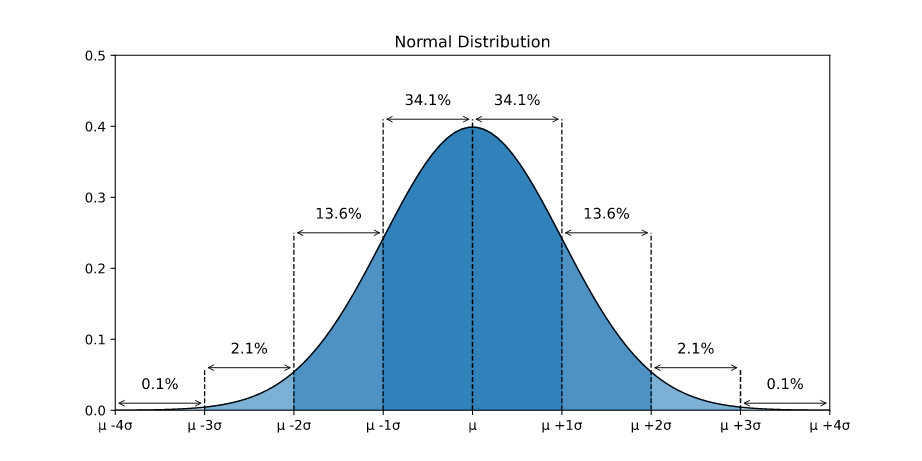
\includegraphics[width = 0.45 \textwidth]{normalele.png}
        \caption{Exemplificació d'una distribució normal.}
        \label{fig:my_label}
    \end{figure}

    \item La complexitat dels mètodes són d'ordre lineal; és a dir, $O(n)$ (on $n$ és el nombre de mostres que volem que generi el programa).
    \item Aconsellem llegir el document d'utilització de la llibreria \textcolor{LimeGreen}{integracio.h} i del fitxer $gauss.c$ per informació complementaria sobre l'ús i les propietats del programa ja que són utilitzats durant l'execució del shell script $comprovador.sh$.
    \item Recalcar que al tractar-se el fitxer $comprovador.sh$ d'un arxiu $bash$, l'execució del mateix (a l'hora de fer tots els càlculs i crides als subprogrames amb una $n$ prou gran) sol trigar una quantitat de temps significativa.
\end{itemize}
\end{document}
